\section{Scalability}
\label{sec:scalability}

It's common for lotteries to have millions of participants. Their large scale is an important characteristic, so it's natural to explore the scalability of our implementation. While the Ethereum platform has no problem with having connections to participants all over the world, it has a limited amount of transactions that can be processed per time unit. Even if transaction costs can be overcome by making them low relative to ticket prices, the limit on transaction throughput will stay the same. The stakes involved in the lottery will also get higher the more participants join. This fact might create incentives for miners to censor transactions and is covered in \ref{sec:censorship}.

\subsection{Transaction throughput}

Our lottery has clearly defined limits for the amount of transactions that need to be made for each participant. The amount of transactions of each type and its average gas usage is listed in \ref{tab:gas-usage}. Setting up the lottery requires $2N$ transactions, each participant joining takes one transaction, playing each match takes at most $4$ transactions, and the winner needs a single transaction to withdraw the prize. So the maximum amount of transactions for a successful lottery will be $7N-1$.  
The time interval in which the transactions need to be made is important, as the intensity of transaction demand will vary during the lifecycle of the lottery. We expect a ticket purchasing period that lasts for several days where the demand for transactions will not be high per time unit. When the matches on the first level can be played, we have $N/2$ matches that all need to be interacted with at the same time. If the time interval between match phases of these matches is too low, the blockchain will not be able to handle all the transactions that need to be made. The demand for transactions after the first match will exponentially decrease for each level as the amount of matches is halved for each level in the tournament tree.

The amount of participants is $2^L$ and there are $2^{l-1}$ matches for each level if we count $l$ from $L$ at the first level matches to $1$ for the final match. The commit phase and reveal phase for each match require two transactions each. The amount of transactions needed for each phase at each level will then be $txs\_phase_{l}=2 \cdot 2^{l-1}=2^l$ – one for each remaining player. Ethereum has a transaction throughput capacity of some amount of transactions per block $tpb$. Since blocks are mined on average at a fixed rate, transactions per block is equivalent to transactions per time unit.
Each phase in a match lasts for a number of blocks $td$ which is set when each match contract is deployed. For it to be theoretically possible to perform all the transactions for each match, $td$ must be set so that $td > \frac{2^{l}}{tpb}$.

Ethereum currently has about $150$ transactions per block. Using this value for $tpb$, we can chart some values of what $td$ ought to be in the first level matches for various amounts of participants.

\begin{table}[h]
\centering
\caption{Estimates of $td$ if all transactions on the blockchain are used for our lottery.}
\label{tab:td-100percent-transactions}
\begin{tabular}{|l|l|l|l|l|}
\hline

N & td & td in s & td in m & td in h \\ \hline
256 & 2 & 30 & 0,5 & 0,01 \\ \hline
1024 & 7 & 105 & 1,8 & 0,03 \\ \hline
4096 & 28 & 420 & 7,0 & 0,12 \\ \hline
16384 & 110 & 1650 & 27,5 & 0,46 \\ \hline
65536 & 437 & 6555 & 109,3 & 1,82 \\ \hline
131072 & 874 & 13110 & 218,5 & 3,64 \\ \hline
262144 & 1748 & 26220 & 437,0 & 7,28 \\ \hline
1048576 & 6991 & 104865 & 1747,8 & 29,13 \\ \hline

\end{tabular}
\end{table}

\begin{table}[h]
\centering
\caption{Estimates of $td$ if 10\% of the transactions on the blockchain are used for our lottery.}
\label{tab:td-10percent-transactions}
\begin{tabular}{|l|l|l|l|l|}
\hline

N & td & td in s & td in m & td in h \\ \hline
256 & 18 & 270 & 4,5 & 0,08 \\ \hline
1024 & 69 & 1035 & 17,3 & 0,29 \\ \hline
4096 & 274 & 4110 & 68,5 & 1,14 \\ \hline
16384 & 1093 & 16395 & 273,3 & 4,55 \\ \hline
65536 & 4370 & 65550 & 1092,5 & 18,21 \\ \hline
131072 & 8739 & 131085 & 2184,8 & 36,41 \\ \hline
262144 & 17477 & 262155 & 4369,3 & 72,82 \\ \hline
1048576 & 69906 & 1048590 & 17476,5 & 291,28 \\ \hline

\end{tabular}
\end{table}

\begin{table}[h]
\centering
\caption{Time for the entire lottery if 10\% of the transactions on the blockchain are used for our lottery.}
\label{tab:total-time-10percent-transactions}
\begin{tabular}{|l|l|l|l|l|}
\hline

N & td & time in s & time in m & time in h \\ \hline
256 & 73 & 1095 & 18,3 & 0,30 \\ \hline
1024 & 279 & 4185 & 69,8 & 1,16 \\ \hline
4096 & 1100 & 16500 & 275,0 & 4,58 \\ \hline
16384 & 4378 & 65670 & 1094,5 & 18,24 \\ \hline
65536 & 17487 & 262305 & 4371,8 & 72,86 \\ \hline
131072 & 34964 & 524460 & 8741,0 & 145,68 \\ \hline
262144 & 69917 & 1048755 & 17479,3 & 291,32 \\ \hline
1048576 & 279634 & 4194510 & 69908,5 & 1165,14 \\ \hline

\end{tabular}
\end{table}

The most realistic scenario is that only a small ratio of all the transactions in a block are used for the lottery. We also see that for a lottery of any size, there will probably be quite high demand for transactions, which will in turn raise gas prices. This has implications for what the minimum viable ticket price should be, as it cannot be assumed that the gas price will be low for the first level of the lottery unless $td$ is very high.

Although $td$ can be set arbitrarily high, we probably don't want the lottery to drag on for weeks before a winner is determined. It seems like the lottery will face scalability issues in the order of 100000s or from $2^{17}$ participants if we want to complete it within days. The number of transactions needed will decrease exponentially with higher levels, so the first two levels will account for 75\% of the total time of the playing phase. 

There are plans for Ethereum to increase the number of transactions it can handle by implementing proof-of-stake and sharding. While this might make our lottery capable of handling more participants, we don't know whether such a change in the protocol might introduce a new threat model that makes the lottery less scalable in other ways.

\subsection{Transaction costs and max prize}

Due to the size of the prize increasing linearly with the number of participants, a censorship attack by miners gets more profitable the more participants there are, which puts a limit on scalability. Even if a censorship attack is unlikely to succeed, it cannot be ignored when it can give high rewards to dishonest miners. Since the lottery prize is decided by the ticket price as well as the number of participants, the ticket price can be set so low that the total prize is not high enough to encourage manipulation by miners. The ticket price is however bounded to minimum value where the transaction costs for participating exceed the ticket price itself.

Figure \ref{fig:cost-ratio-chart} shows the ratio of the ticket price going to transaction costs as a function of number of participants and a max tolerable prize. Figure \ref{fig:prize-chart} show the prize for the lottery for a given number of participants and ratio of transactions costs to ticket price. Both assume a gas price of 1.5 gwei.
The charts show us the maximum scale of the lottery under different conditions for maximum tolerable prize and ticket price going to transaction costs. With the generous assumptions that the transaction costs can be as much as 40\% of the ticket price, and the maximum prize being 900 ether, this scalability limit approaches that of the above analysis of transaction throughput.

Figure \ref{fig:price-chart} shows the transaction cost to ticket price ratio on the left y-axis which the thick blue line plots. The right y-axis shows the total prize for a given ticket price and is plotted by multiple thin lines that each represent a specific number of participants. The chart gives some idea of which tickets prices can be used for different amounts of participants and different maximum prizes. For instance, if a cost ratio of 0.1 is required, the thick blue line indicates that the ticket price will be slightly less than 0.3 ETH. At that price, only lotteries with less than $32768=2^{15}$ will have a prize of less than 1000 ETH. If we start from the other direction and consider a lottery with $8192=2^{13}$ participants, plotted by the thin pink line, it can handle ticket prices of slightly more than 0.1 ETH if the prize is to be less than 1000 ETH, and a ticket price of 0.06 if the prize is to be below 500 ETH. Furthermore, it shows that lotteries with few participants can handle quite high ticket prices without risking too much exposure by a high prize, while lotteries with more than $2^{16}$ participants can barely handle ticket prices so low that the cost ratio is nearly prohibitive unless a very large prize is acceptable.

The calculations in the charts do not account for the organizer probably taking some portion of the prize as a fee. Accounting for that would reduce the total prize, but would correspondingly increase the cost of buying tickets from the participants' perspective.


\begin{figure}[htbp]
  \centering
  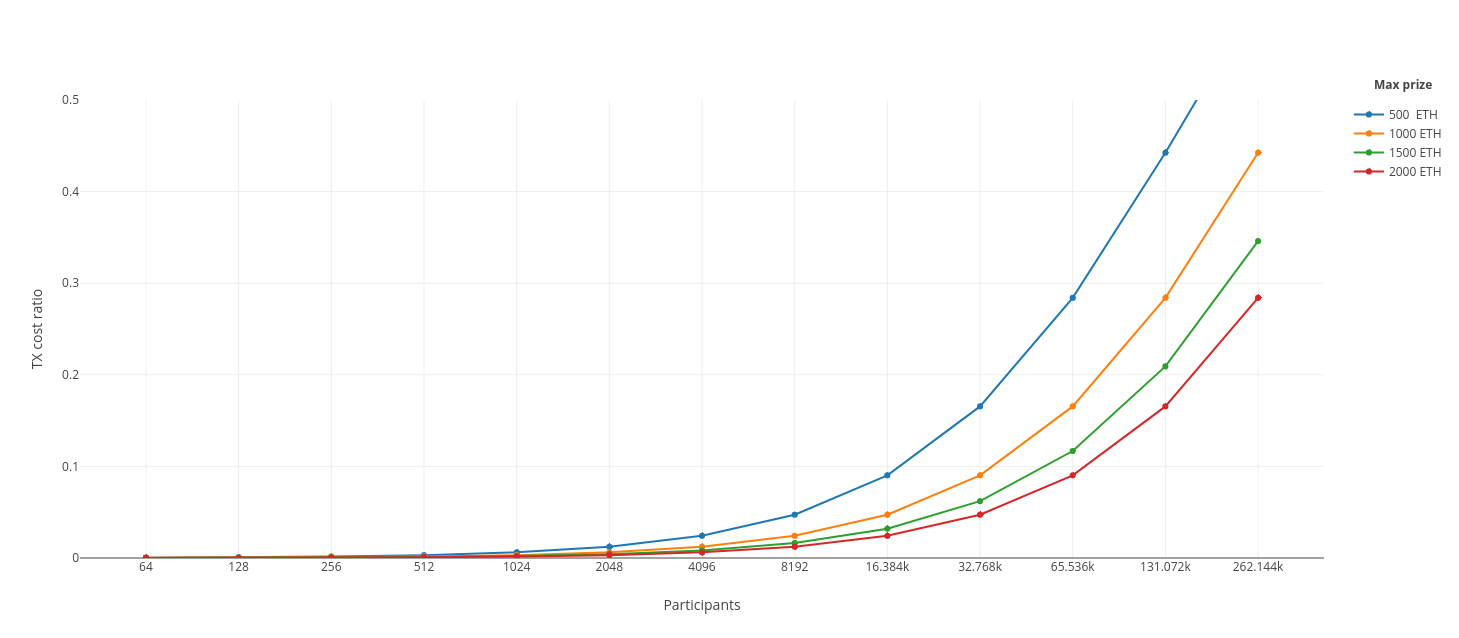
\includegraphics[width=\columnwidth]{figures/max_participants_cost_ratio.png}
  \caption{Cost ratio as a function of participants and max prize.}
  \label{fig:cost-ratio-chart}
\end{figure}

\begin{figure}[htbp]
  \centering
  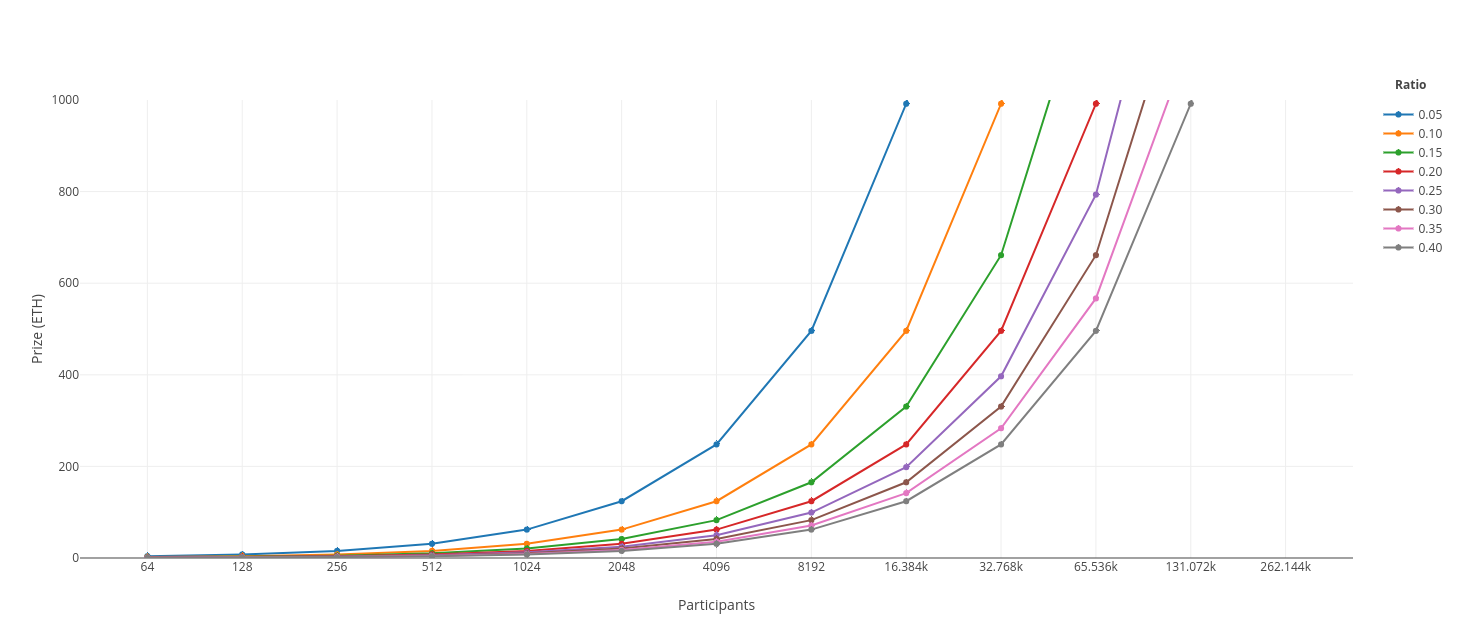
\includegraphics[width=\columnwidth]{figures/max_participants_prize.png}
  \caption{Prize as a function of participants and cost ratio.}
  \label{fig:prize-chart}
\end{figure}

\begin{figure}[htbp]
  \centering
  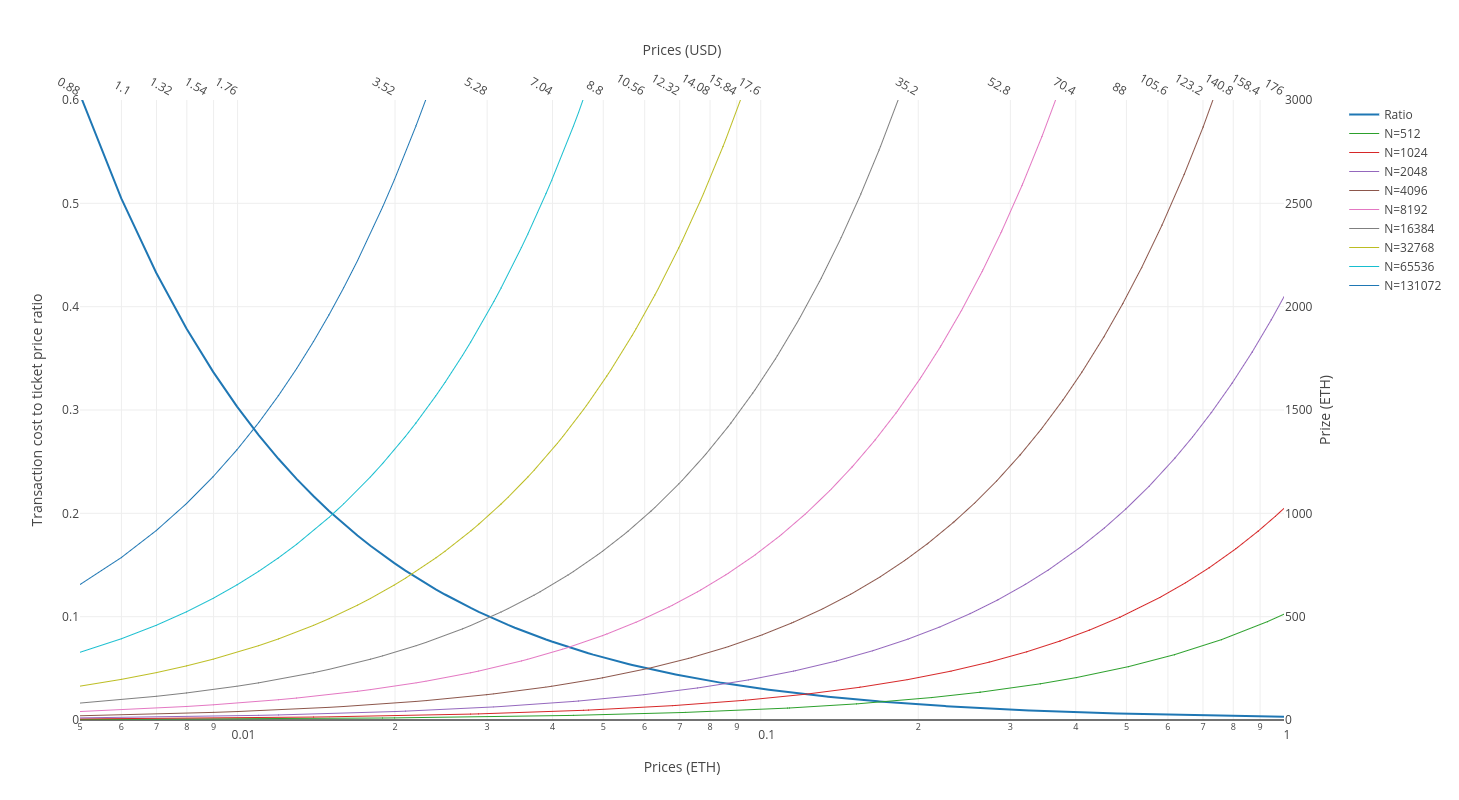
\includegraphics[width=\columnwidth]{figures/ticket_prices.png}
  \caption{Cost ratio and prize as a function of participants and ticket price.}
  \label{fig:price-chart}
\end{figure}
